\documentclass[a4paper]{article}

\usepackage{fullpage} % Package to use full page
\usepackage{parskip} % Package to tweak paragraph skipping
\usepackage{tikz} % Package for drawing
\usepackage{amsmath}
\usepackage{hyperref}
\usepackage{enumitem}

\title{Data Mining: Homework 1}
\author{Anxhelo Xhebraj \\
        \href{mailto:xhebraj.1643777@studenti.uniroma1.it}{\texttt{xhebraj.1643777@studenti.uniroma1.it}}
        }
\date{\{7..21\} Oct 2018}

\begin{document}

\maketitle

\subsection*{Problem 1}
We shuffle a standard deck of cards, obtaining a permutation that is uniform over all $52!$ possible permutations.
\begin{enumerate}
    \item Define a proper probability space $\Omega$ for the above random process.  What is the probability
of each element in $\Omega$? \\ \\
         \textbf{Solution}: \iffalse Let $c := (rank, suit) \in \{A,2, ..., J, Q, K\} \times \{Hearts, Spades, Diamonds, Clubs\}$ represent a card of the deck. \fi We can define $\Omega$ as the set of all the permutations of the cards. Given that the cards are 52 then $ |\Omega| = 52!$ and with all the permutations being equiprobable then $\forall \omega \in \Omega, Pr(\omega) = \frac{1}{52!}$
    \item Find the probability of the following events:
        \begin{enumerate}
            \item The first two cards include at least one ace. \\ \\
            \textbf{Solution}: Denote by $c_1$, $c_2$ the first and second card in the permutation. We have that $Pr(\{c_1.rank = A, c_2.rank = A\}) = 1 - Pr(c_1.rank \neq A, c_2.rank \neq A)$. The latter probability is equal to the sum of the probabilities of all permutations having no Ace in the first two cards which are all equiprobable simple events. The number of such permutations can be counted as follows. From all the cards except aces we choose two cards which will be the first two ($\binom{48}{2}$ possible combinations). Depending by the order we choose them we get a different permutation thus we must multiply by the number of permutations of the chosen cards which are 2! and the number of permutations of the remaining 50 cards being 50!. With all cards permutations being equiprobable then
            \begin{align*}
                Pr(\{c_1.rank = A, c_2.rank = A\}) &= 1 - Pr(c_1.rank \neq A, c_2.rank \neq A) \\
                                                   &= 1 - \frac{1}{52!} \binom{48}{2} 2! \cdot 50! \\
                                                   &= \frac{33}{221} \approx 0.1493
            \end{align*}
            
            \item The first five cards include at least one ace. \\ \\
            \textbf{Solution}: Extending the reasoning above to the first five cards we can conclude
            \begin{align*}
                Pr(\exists i \in \{1..5\}: c_i.rank = A) &= 1 - Pr(\forall i \in \{1..5\} \Rightarrow c_i.rank \neq A) \\
                                                         &= 1 - \frac{1}{52!}\binom{48}{5}5!\cdot 47! \\
                                                         &= \frac{18472}{54145} \approx 0.3412
            \end{align*}
            
            \newpage
            
            \item  The first two cards are a pair of the same rank (they are the same number or both are
J, or both are Q, etc.) \\ \\
            \textbf{Solution}: We must count the number of card permutations having at its start two cards of the same rank. We first have to choose which rank among 13. Then what suit to assign to each of the two cards producing $\binom{4}{2} 2!$ possibilities and finally the ordering of the remaining 50 cards.
            \begin{align*}
                Pr(c_1.rank = c_2.rank) &= \frac{1}{52!} 13 \binom{4}{2} 2! \cdot 50! \\
                                        &= \frac{3}{51} \approx 0.0588
            \end{align*}
            
            \item The first five cards are all diamonds. \\ \\
            \textbf{Solution}: All the card permutations having in the first five cards all diamonds can be counted as: $\binom{13}{5}$ the possible ranks of the first 5 cards times 5! 47! which are the possible orderings of the first 5 cards and the remaining 47
            \begin{align*}
                Pr(\forall i \in \{1..5\} \Rightarrow c_i.suit = Diamonds) &= \frac{1}{52!} \binom{13}{5} 5! \cdot 47! \\
                &= \frac{1287}{2598960} \approx 0.0005
            \end{align*}
            
            \item  The first five cards form a full house (three of one rank and two of another rank). \\ \\
            \textbf{Solution}: The number of permutations having a full house in the first five cards is $13\binom{4}{3}$ which is the number of ways we can choose the suits for the 3 cards of the same rank and the rank of such cards, times $12\binom{4}{2}$ which is the number of ways we can choose the suits for the other 2 cards of the same rank and the rank of such cards given that must be different from the previous one. Finally we can reorder the first 5 cards and the remaining 47 as we wish therefore we must multiply such number by 5! and 47!
            \begin{align*}
                E &= \text{"Full house in first five cards"} \\
                Pr(E) &= \frac{1}{52!} 13 \binom{4}{3} 12 \binom{4}{2} \cdot 5! \cdot 47! \\
                      &= \frac{6}{4165} \approx 0.0014
            \end{align*}
            
        \end{enumerate}
\end{enumerate}

\subsection*{Problem 2}

A group of $n$ men and $m$ women go to a Chinese restaurant and sit in a round table,
such that each person has two other persons next to him/her.

\begin{enumerate}
    \item  Describe a sample space that describes the random process. \\ \\
    \textbf{Solution}: First we assign an identifier to each man and woman. Thus the set of man is $\{M_i, \forall i \in \{1..n\}\}$ and woman $\{W_i, \forall i \in \{1..m\}\}$. We can define a first seat in the table and produce a sequence of $M_k$s and $W_j$s
    depending whether the person in the corresponding seat is a Man or a Woman. The number of possible unique
    sequences, and thus the cardinality of the sample space, is $(n+m)!$ and all simple events are equiprobable with $Pr(\omega) = \frac{1}{(n+m)!},\text{ } \forall \omega \in \Omega$.
    \newpage
    \item  Find the expected number of men who will be sitted next to at least one woman. \\ \\
    \textbf{Solution}: First we define a Bernoulli random variable $X_i$ for each man $i$ such that
    \begin{align*}
    X_i =
    \begin{cases}
        1 & \text{if $M_i$ sits next to at least one woman} \\
        0 & \text{if $M_i$ sits next to two men}
    \end{cases}
    \end{align*}
    \iffalse
    We can write the probability of $X_i = 1$ as 1 minus the probability of a man sitting next to two man (the complementary of the event a man sits next to at least one woman). Let $t_k$ be the $k$-th seat in the table then for any $k, i$
    \begin{align*}
        Pr(X_i = 1) &= 1 - Pr(t_{k - 1} = M, t_{k + 1} = M | t_k = M) \\
        &= 1 - Pr(t_{k-1} = M | t_k = M) \cdot Pr(t_{k+1} = M | t_k = M, t_{k - 1} = M) \\ 
        &=
        \begin{cases}
            0 & n = 0 \text{\quad or \quad} m = 0\\
            1 & m = 1 \text{\quad and \quad} n = 1 \\
            1 - \frac{n-1}{n+m-1} \cdot \frac{n-2}{n+m-2} & n + m > 2 \text{\quad and \quad} n \neq 0, m \neq 0\\
        \end{cases}
    \end{align*}
    \fi
    We can write the probability of $X_i = 1$ as $1-Pr(X_i = 0)$. $Pr(X_i = 0)$ can be defined as sum of the probabilities of simple events which can be counted as the product of: $(n + m)$ which are the number of seats $M_i$ can sit; $\binom{n-1}{2}2!$ the combinations of man that can sit at his sides considering their order; $(n+m-3)!$ the possible ways the other participants can sit. Moreover we must treat edge cases properly as follows.
    \begin{align*}
        Pr(X_i = 0) &= \frac{1}{(n + m)!} \cdot (n+m)\binom{n-1}{2}2!(n+m-3)! \\
                &= \frac{n-1}{n+m-1} \cdot \frac{n-2}{n+m-2} \\ \\
        Pr(X_i = 1) &=
        \begin{cases}
            0 & n = 0 \text{\quad or \quad} m = 0\\
            1 & m = 1 \text{\quad and \quad} n = 1 \\
            1 - Pr(X_i = 0) & n + m > 2 \text{\quad and \quad} (n \neq 0 \text{ or } m \neq 0)\\
        \end{cases}
    \end{align*}

    \begin{align*}
        \mathbb{E}\Big[\sum_{i = 1}^{n} X_i \Big] &= \sum_{i = 1}^{n} \mathbb{E}[X_i] \text{ \quad(by linearity of expectation)} \\
        &= n\cdot Pr(X_i = 1)
    \end{align*}
\end{enumerate}

\subsection*{Problem 3}

The Erdos-Renyi $G_{n,p}$ random-graph model is a mathematical model for creating
random graphs. Fix a positive integer $n$ and a value $p \in [0, 1]$, then a graph created according
to the $G_{n,p}$ model, has $n$ nodes, and each pair of distinct nodes is connected with an edge with
probability $p$; all pairs being independent from each other.

\begin{enumerate}
    \item Define an appropriate probability space $\Omega$ to describe the $G_{n,p}$ model. What is
    its size? \\ \\
    \textbf{Solution}: The sample space of the problem can be defined in terms of presence and absence
    of edges in the graph with respect to all possible edges. The set of edges of all graphs produced by
    the model is always a subset of the "most dense" graph having $\frac{n(n-1)}{2}$ edges. Therefore for
    each graph we can define a vector of $\frac{n(n-1)}{2}$ positions where each position represents an edge of the "most dense" graph with value 1 if it is present in this sample or 0 otherwise. The number of such possible distinct vectors is $|\Omega| = 2^\frac{n(n-1)}{2}$
    
    \item What is the probability of each element of $\Omega$? \\ \\
    \textbf{Solution}: Since all pairs are independent we can find the probability as the probability that a graph has exactly $|E|$ edges i.e. $p$ to the power of
    the number of edges present in the graph times $(1-p)$ to the power of edges missing in the graph.
    \begin{align*}
     Pr(\omega) &= p^{\sum \omega[i]} \cdot (1-p)^{\frac{n(n-1)}{2} - \sum \omega[i]}, \text{}
           \forall \omega \in \Omega
    \end{align*}
    where $\sum \omega[i]$ is the sum of the entries of the vector i.e. the number of edges of the graph.
    
    \item What is the probability that a graph created according to
$G_{n,p}$ contains exactly two cycles of size $\frac{n}{2}$ and no other edges (assume that $n$ is even for this)? A cycle is a sequence of vertices $v_1,v_2, ..., v_l, v_1$ ($l \geq 3$), with $v_i \neq v_j$ for $i,j \in \{1,...,l\}$ such that each edge $(v_i, v_{i+1})$ exists in the graph (as well as $(v_l, v_1)$). \\ \\
    \textbf{Solution}: We have to count the number of simple events $\omega \in \Omega$ such that
    there are exactly two cycles of size $n/2$ and then sum their probabilities (which are the same given that they have the same number of edges). First there are $\binom{n}{n/2}$ ways we can split the set of nodes into two sets each forming a cycle. Moreover given a set of $n/2$ nodes there are $\frac{(n/2)!}{2 \cdot n/2}$ possible ways we can link them to form a cycle ($(n/2)!$ permutations of the nodes but $2 \cdot n/2$ permutations are just rotations of other permutations or obtained by inverting the order of the nodes\footnote{Suppose 4 nodes $A,B,C,D$. The circle $ABCD$ is the same as $DCBA$ (inversion) and $BCDA$ (rotation). There are 4 rotations and for each rotation its inversion.}). The latter number should be counted for each cycle. Finally since the probability of a graph depends only by the number of its edges which in this case are $n/2 \cdot 2$ (each cycle has $n/2$ edges), we have that
    \begin{align*}
        E &= \text{"Only two cycles of size $n/2$ and no other edges"} \\
        Pr(E) &= \bigg( p^{\frac{n}{2}\cdot2} (1-p)^{\frac{n(n-1)}{2} - \frac{n}{2}\cdot2} \bigg) \binom{n}{n/2} \bigg( \frac{(n/2)!}{2 \cdot n/2} \bigg)^2
    \end{align*}
    
    \item  What is the probability that a graph created according to $G_{n,p}$ contains exactly
    two cycles of any size and no other edges? \\ \\
    \textbf{Solution}: We can extend the reasoning above first finding the probability of a graph having only 2 cycles, one of size $k$ and the other of size $j$
    \begin{align*}
        E_{\{k,j\}} &= \text{"Only two cycles, one of size $k$ and the other $j$,  and no other edges"} \\
        Pr(E_{\{k,j\}}) &= \bigg( p^{(k + j)} (1-p)^{\frac{n(n-1)}{2} - (k + j)} \bigg) \binom{n}{k} \bigg( \frac{k!}{2k} \bigg) \binom{n-k}{j} \bigg( \frac{j!}{2j} \bigg)
    \end{align*}
    then summing over all possible $k,j$ with the former ranging from 3 up to $\lfloor \frac{n}{2} \rfloor$ (the case $k = \lfloor \frac{n}{2} \rfloor + i$ meaning a cycle of size $\lfloor \frac{n}{2} \rfloor + i$ and the other of $j = l < k$ has already been counted in $j = \lfloor \frac{n}{2} \rfloor + i$ and $k = l$). Since $E_{\{k,j\}} \cap E_{\{i, l\}} = \emptyset$, $\forall k \neq i, j \neq l$ (i.e. disjoint)
    \begin{align*}
        E &= \text{"Only two cycles of any size"} 
    \end{align*}
    \begin{align*}
        Pr(E) &= Pr\bigg( \bigcup_{k = 3}^{\lfloor \frac{n}{2} \rfloor} \bigcup_{j = k}^{n - k} E_{\{k,j\}} \bigg) \\
        &= \sum_{k = 3}^{\lfloor \frac{n}{2} \rfloor} \sum_{j = k}^{n - k} \bigg( p^{(k + j)} (1-p)^{\frac{n(n-1)}{2} - (k + j)} \bigg) \binom{n}{k} \bigg( \frac{k!}{2k} \bigg) \binom{n-k}{j} \bigg( \frac{j!}{2j} \bigg)
    \end{align*}

    \item  In a graph created by the $G_{n,p}$ model, what is the expected degree of a node? \\ \\
    \textbf{Solution}: For each pair of nodes $(i,j)$ we define a Bernoulli random variable as follows
    \begin{align*}
    X_{i,j} =
    \begin{cases}
        1 & \text{if edge $(i,j)$ is present in the graph} \\
        0 & \text{otherwise}
    \end{cases}
    \end{align*}
    By the definition of the model we have that $Pr(X_{i,j} = 1) = p$, thus $\forall i \in \{1..n\}$.
    \begin{align*}
        \mathbb{E}[deg(i)] &= \mathbb{E}\Big[ \sum_{j \in \{1..n\}: j \neq i} X_{i,j} \Big] \\
        &= \sum_{j \in \{1..n\}: j \neq i} \mathbb{E}[X_{i,j}] & (\text{by linearity of expectation}) \\
        &= (n - 1) \cdot p
    \end{align*}

    \item In a graph created by the $G_{n,p}$ model, what is the expected number of edges? \\ \\
    \textbf{Solution}: We can count the edges of a graph by summing for each node its degree and divide such number by $2$ since we count each edge twice (once from one node and another by the other node).
    \begin{align*}
        \mathbb{E}\big[|E|\big] &= \mathbb{E}\Bigg[ \frac{1}{2} \sum_{i = 1}^{n} deg(i) \Bigg] \\
        &= \frac{1}{2} \sum_{i = 1}^{n} \mathbb{E}[deg(i)] & \text{(by linearity of expectation)}\\
        &= \frac{1}{2} \sum_{i = 1}^{n} (n-1)p & \text{($\mathbb{E}[deg(i)] = (n-1)p$ $\forall i$)} \\
        &= \frac{n(n-1)}{2} \cdot p
    \end{align*}

    \item We  define a house subgraph to be a subgraph of 5 nodes, $\{v_1, ... ,v_5\}$ in which the
    edges $\{v_1,v_2\}$, \\ $\{v_1,v_3\}$, $\{v_2,v_3\}$,$\{v_2,v_4\}$,$\{v_3,v_5\}$,$\{v_4,v_5\}$
    exist, and no other edge between them exists (see Figure \ref{house}). What is the expected number of
    house subgraphs in a random graph according to $G_{n,p}$ ?
    \begin{figure}[!htbp]
    \begin{center}
    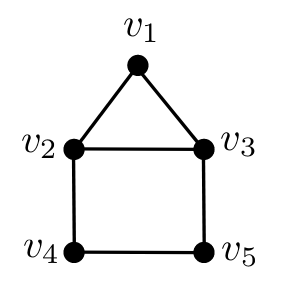
\includegraphics[width=70pt]{house.png}
    \end{center}
    \caption{\textit{The house subgraph}}\label{house}
    \end{figure}
    \\
    \textbf{Solution}: First we must find out in how many ways we can arrange 5 nodes to form a house. We have $\binom{5}{3}$ possible ways to choose the 3 vertices out of the 5 that will form the roof of the house. If we label positions from left to right (following Figure \ref{house} $v_2$ has position 1, $v_1$ position 2 and $v_3$ position 3) the order in which we place the 3 vertices also produces a different house, thus we must multiply by $3!$. Finally the remaining two positions are fixed since swapping them is already considered in the possible positions of the vertices of the roof.
    \[ \text{Number of house arrangements given 5 nodes} = \binom{5}{3}3! \]
    Each arrangement has probability $p^6(1-p)^{\frac{5\cdot4}{2} - 6}$ (i.e. the probability of having 6 edges) and it's disjoint from the others. Thus, given a graph in $G_{n,p}$, we can define a Bernoulli random variable $X_i$ for each possible subset of size 5 of its nodes such that
    \begin{align*}
    X_i =
    \begin{cases}
        1 & \text{if subset $i$ forms a house} \\
        0 & \text{otherwise}
    \end{cases}
    \end{align*}
    with $Pr(X_i = 1) = p^6(1-p)^{4}\binom{5}{3}3!$, $\forall i$ \\
    Finally we can calculate the expected value by summing over all possible groups of 5 nodes of the graph
    \begin{align*}
        \mathbb{E}\Bigg[ \sum_{i = 1}^{\binom{n}{5}} X_i \Bigg] &= \sum_{i = 1}^{\binom{n}{5}} \mathbb{E}[X_i] & (\text{by linearity of expectation}) \\
        &= \sum_{i = 1}^{\binom{n}{5}} Pr(X_i = 1) \\
        &= \binom{n}{5} p^6(1-p)^{4}\binom{5}{3}3!
    \end{align*}
\end{enumerate}

\end{document}